\chapter{Introducci\'on}
\label{sec:intro}

La {\bf generaci\'on de lenguaje natural (GLN)} es el proceso autom\'atico (o semi autom\'atico) de construcci\'on de un texto en lenguaje natural para la comunicaci\'on con fines espec\'ificos. Este proceso que convierte informaci\'on a texto en lenguaje natural es \'util para aplicaciones pr\'acticas en las que, por ejemplo, es necesario hacer accesible grandes vol\'umenes de informaci\'on posiblemente t\'ecnica. La GLN se ha usado para generar recomendaciones de restaurantes personalizadas, para resumir informaci\'on m\'edica, para generar pron\'osticos del clima, entre otros~\cite{dale2000}. La generaci\'on de lenguaje natural, est\'a dentro del \'area de procesamiento del lenguaje natural, que es una rama principal de la inteligencia artificial.

En el marco de esta tesis, una {\bf expresi\'on referencial (ER)} es un sintagma nominal que identifica un\'ivocamente a un objeto en un contexto y para un interlocutor particular. Si quisi\'eramos referirnos al objeto se\~nalado por la flecha en la Figura~\ref{GRE3D7-stimulus1}, podr\'iamos hacerlo con alguna de las expresiones referenciales que se muestran en la Figura \ref{er-figura1}.

\begin{figure}[h]
\begin{subfigure}{.5\textwidth}
  \centering
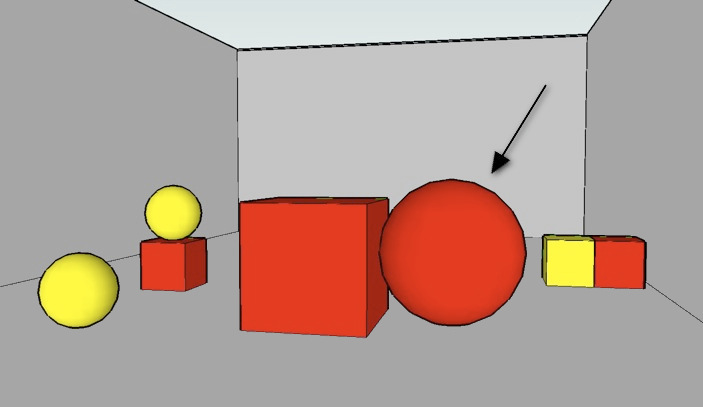
\includegraphics[width=\textwidth]{images/22sinletrasClaro.jpg}
  \caption{}\label{GRE3D7-stimulus1}
\end{subfigure}%
\begin{subfigure}{.5\textwidth}
 \centering
\begin{tabular}{l}
 {\it La esfera grande}\\

 {\it La esfera roja que est\'a al lado del cubo rojo} \\

 {\it El objeto que est\'a al lado del cubo grande}\\

 {\it La bola roja}\\

 {\it La pelota a la izquierda del cubo amarillo}\\

 {\it La bola grande}\\

 {\it La esfera que est\'a a la derecha del cubo rojo y a }\\
{\it la izquierda del cubo amarillo}\\

 {\it La cosa que est\'a a la derecha del cubo del medio}\\

  {\it ...}
 \end{tabular}
\hspace*{-30cm}
\centering\caption{}\label{er-figura1}
\end{subfigure}
\begin{centering}
\caption{En (b) se listan expresiones referenciales que identifican un\'ivocamente al objeto se\~nalado por la flecha en la escena ilustrada en (a).}
\label{figura-er}
\end{centering}
\end{figure}

La \textbf {generaci\'on de expresiones referenciales (GER)} entre todas las subtareas de GLN, es una de las que ha recibido m\'as atenci\'on. En la pr\'actica, la mayor\'ia de los sistemas de GLN, con independencia de su finalidad, contiene un m\'odulo de GER de alg\'un tipo~\cite{Mellish2004}. Esto no es sorprendente
en vista del papel central que las expresiones referenciales tienen en la comunicaci\'on. Un sistema que proporciona
consejos sobre los viajes a\'ereos \cite{white2010generating} tiene que hacer referencia a los vuelos ---{\it el vuelo m\'as barato}, {\it un vuelo directo}---, un sistema de navegaci\'on para autom\'oviles~\cite{Drager:2012:GLN:2380816.2380908}
necesita generar descripciones espaciales ---{\it tomar el puente junto a la iglesia, a la derecha}---,
y un robot que ensambla piezas de juguetes junto con un usuario humano~\cite{foster-etal-ijcai2009} debe hacer referencia a los componentes ---{\it inserte el perno verde hasta el final en el cubo rojo}. Cuando hablamos, nos referimos a cosas (tangibles como un puente, o intangibles como una fecha), es decir generamos expresiones referenciales. Un sistema que genera texto, tambi\'en deber\'a generar expresiones referenciales. La generaci\'on autom\'atica de expresiones referenciales es el tema de esta tesis.

Un sistema de GLN incluye 3 etapas: {\bf determinaci\'on de contenido} ---qu\'e decir--- {\bf lexicalizaci\'on} ---con qu\'e palabras--- y {\bf realizaci\'on ling\"{u}\'istica} ---c\'omo decirlo. La determinaci\'on de contenido, elige qu\'e informaci\'on incluir en la oraci\'on. La lexicalizaci\'on elige qu\'e lexemas usar para comunicar el contenido determinado por la etapa anterior. Y la realizaci\'on arma la oraci\'on agregando los art\'iculos, preposiciones, y dem\'as palabras funcionales necesarias y orden\'andolas de forma tal que la frase resultante sea gramaticalmente aceptable. 

Un sistema de GER, tiene esas 3 etapas tambi\'en: {\bf determinaci\'on de contenido} ---decide qu\'e propiedades o relaciones del objeto a describir se incluir\'an en la expresi\'on referencial--- {\bf lexicalizaci\'on} ---elige las palabras que se van a usar para nombrar las propiedades y relaciones--- y {\bf realizaci\'on ling\"u\'istica} ---se encarga de armar el sintagma nominal para que sea gramaticalmente correcto.

Por ejemplo, la primer ER de la Figura \ref{figura-er} incluye las propiedades {\it tama\~no} y {\it forma} del objeto se\~nalado por la flecha, lexicalizadas como {\it grande} y {\it esfera} respectivamente y realizadas agregando el art\'iculo {\it la} antes de {\it esfera}, e incluyendo el sustantivo {\it esfera} antes que el adjetivo {\it grande}; formando as\'i el sintagma nominal {\it la esfera grande} que es correcto en espa\~nol. Otra lexicalizaci\'on y realizaci\'on de las mismas propiedades ---es decir, de la misma sem\'antica--- podr\'ia ser {\it la bola de gran tama\~no}. A lo largo de esta tesis usaremos el t\'ermino {\bf expresi\'on referencial (ER)} para nombrar la salida de cualquiera de las 3 etapas de la GER. Es decir, llamaremos expresi\'on referencial al conjunto de propiedades y relaciones que refieren un\'ivocamente a un objeto aunque no est\'en lexicalizadas o realizadas.

En esta tesis nos enfocamos en la parte de determinaci\'on de contenido, daremos como salida f\'ormulas de l\'ogica que van a determinar el contenido de la ER. En algunos casos se muestran ejemplos que est\'an lexicalizados y realizados, esto se hace a fin de hacer legible e intuitivo el seguimiento de la explicaci\'on.

En lo que sigue introduciremos terminolog\'ia b\'asica, relacionada con la GER que nos servir\'a a lo largo de toda la tesis.

El {\bf dominio} de una ER define los tipos de entidades que est\'an siendo contemplados. Por ejemplo el dominio de la Figura \ref{figura-er} son figuras geom\'etricas en 3 dimensiones. En particular, el dominio incluye cubos y esferas de colores, algunas grandes y otras peque\~nas, situadas en un entorno con perspectiva.

El {\bf contexto} de una ER contiene un subconjunto de las entidades del dominio. La Figura \ref{figura-er} muestra un contexto con 7 entidades del dominio, 4 rojas y 3 amarillas. Otros ejemplos de contextos son los puntos de referencia visibles en un cierto momento en un camino para el que estamos dando direcciones, un subconjunto de las fotograf\'ias utilizadas en una configuraci\'on experimental, o los ingredientes de cocina que ya se han mencionado en una receta. En un dominio visual, el contexto, incluyendo las propiedades de sus objetos y su configuraci\'on espacial, se puede llamar \textbf{escena}. 

Cada {\bf entidad} del contexto (tambi\'en conocido como objeto o elemento) tiene un tipo ---\emph{esfera}--- ciertas propiedades o caracter\'isticas ---\emph{color}---, valores de esas propiedades ---\emph{rojo}---, y puede tener relaciones con otros objetos ---\emph{a la derecha de}. Una {\bf propiedad} (unaria) es una caracter\'istica de una entidad particular. Por ejemplo, la raza de un perro, el tener o no tener bigotes para un hombre, o el color para un objeto. Cada entidad puede tener muchas propiedades, y puede tener {\bf relaciones} (tambi\'en llamadas propiedades binarias), por ejemplo con respecto a la posici\'on f\'isica, como estar situado al lado de otro objeto. 

El {\bf target} (u objetivo), es el subconjunto de objetos de un contexto a los cuales queremos referirnos. En la escena del ejemplo de la Figura \ref{figura-er}, el target es el objeto se\~nalado por la flecha. En este caso, el target es un conjunto singleton, es decir tiene un s\'olo elemento. Si el target tiene m\'as de un elemento, las ERs que lo identifican son plurales.

Dado un contexto, un target y una descripci\'on parcial del target (es decir, una descripci\'on que no lo identifica un\'ivocamente), los {\bf distractores} son otros elementos que se encuentran en el contexto, y que tambi\'en cumplen con la descripci\'on parcial. Por ejemplo, si la descripci\'on parcial es {\it esfera} las esferas que no son el target de la Figura \ref{figura-er} son  distractores, y por ello es necesario seguir agregando propiedades o relaciones para identificar un\'ivocamente al target.

Un {\bf algoritmo} para GER, es un procedimiento autom\'atico que toma, al menos, alg\'un tipo de representaci\'on de un contexto y un target, y da como resultado una (o m\'as) expresi\'on(es) referencial(es) para el target considerado, si puede identificarlo un\'ivocamente en el contexto.

Por ejemplo, una computadora que se enfrenta a la tarea de generar autom\'aticamente expresiones referenciales para la Figura \ref{figura-er} necesitar\'a una representaci\'on de todos los objetos de la figura y las propiedades de cada uno de ellos. En la Figura~\ref{contexto-tabla-propiedades} se muestra una posible forma de representar los objetos, sus propiedades y relaciones: una base de datos que contiene todas las propiedades relevantes de los objetos de la escena. Entonces, la tarea de GER para el objeto $e_5$ involucra encontrar alguna combinaci\'on de valores de propiedades y relaciones con otros objetos, que aplique \'unicamente a $e_5$, y no a los otros objetos. Como dijimos, esta tarea de encontrar las propiedades y relaciones que aplican a un target y no a los distractores, se llama selecci\'on de contenido para la generaci\'on de una expresi\'on referencial. Mirando la Tabla \ref{tabla-propiedades} podemos decir que {\it red ball}, {\it large ball} y {\it large red ball} son algunas ERs del objeto $e_5$, cuyas realizaciones en espa\~{n}ol podr\'ian ser: {\it la bola roja}, {\it la esfera grande} y {\it la esfera grande y roja}. 

\begin{figure}[ht]
%
\begin{subfigure}{.48\textwidth}
  \centering
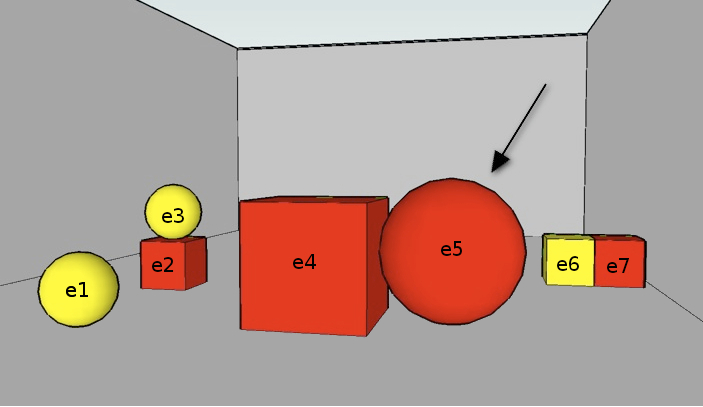
\includegraphics[width=\textwidth]{images/22.jpg}
  \caption{}\label{GRE3D7-stimulus1-ids}
\end{subfigure}
%
\begin{subfigure}{.48\textwidth}
%\hspace*{-15.5cm}
\begin{scriptsize}
\begin{tabular}{|l|c|c|c|c|c|c|c|}
\hline
\textbf {id}& 	\textbf {type}		&	\textbf {color}	&	\textbf {size}& \textbf {right} & \textbf {left} & \textbf {ontop}	& \textbf {below}	\\
   	   &  	    			&	    		&	     		&  \textbf {of}   		 &  \textbf {of}	    &  	&  \\
\hline \hline
$e_1$ & ball & yellow & small & - & - & - & - \\
& & & & & & & \\
$e_2$ & cube & red & small & - & - &- & $e_3$ \\
& & & & & & & \\
$e_3$ & ball & yellow & small & - & - & $e_2$ & -\\
& & & & & & & \\
$e_4$ & cube & red & large & - & $e_5$ & - & -\\
& & & & & & & \\
$e_5$ & ball & red & large & $e_4$ & - & - & -\\
& & & & & & & \\
$e_6$ & cube & yellow & small & - & $e_7$ & - & -\\
& & & & & & & \\
$e_7$ & cube & red & small & $e_6$ & - & - & -\\
\hline
\end{tabular}
\end{scriptsize}
%\vspace*{1cm}
%\center
\centering \hspace*{-8cm} \caption{}\label{tabla-propiedades}
%\end{centering}
\end{subfigure}
\caption{Formalizaci\'on de las propiedades de la escena en una tabla de doble entrada.}\label{contexto-tabla-propiedades}
\end{figure}

En la pr\'oxima secci\'on veremos porqu\'e la tarea de GER es m\'as compleja de lo que parece a primera vista y en la siguiente introduciremos c\'omo herramientas de teor\'ia de modelos nos pueden ayudar.

\section{Expresiones referenciales bajo incertidumbre}
\label{sec:gre-incertidumbre}


Cuando la generaci\'on de expresiones referenciales ocurre en la vida real, en lugar de ocurrir en un experimento controlado, las fuentes de \textbf{incertidumbre} que afectan al proceso se multiplican. En trabajo reciente en el \'area de GER \cite{turner2009,deemter16} se discute que, al intentar usar algoritmos de GER en dominios grandes y realistas (como por ejemplo la descripci\'on de regiones en mapas) la identificaci\'on \'optima del target es una tarea que puede ser aproximada pero raramente lograda. Los autores argumentan que esto se debe, en parte, a que las representaciones geogr\'aficas son necesariamente \textbf{incompletas}. Esta falta de informaci\'on introduce incertidumbre. Por ejemplo, el restaurante se\~nalado por la flecha en la Figura \ref{target_mapa}, ?`es realmente el \'unico restaurante de la calle de C\'adiz o ?`es el \'unico que aparece en el mapa?.

\begin{figure}[h]
\centering
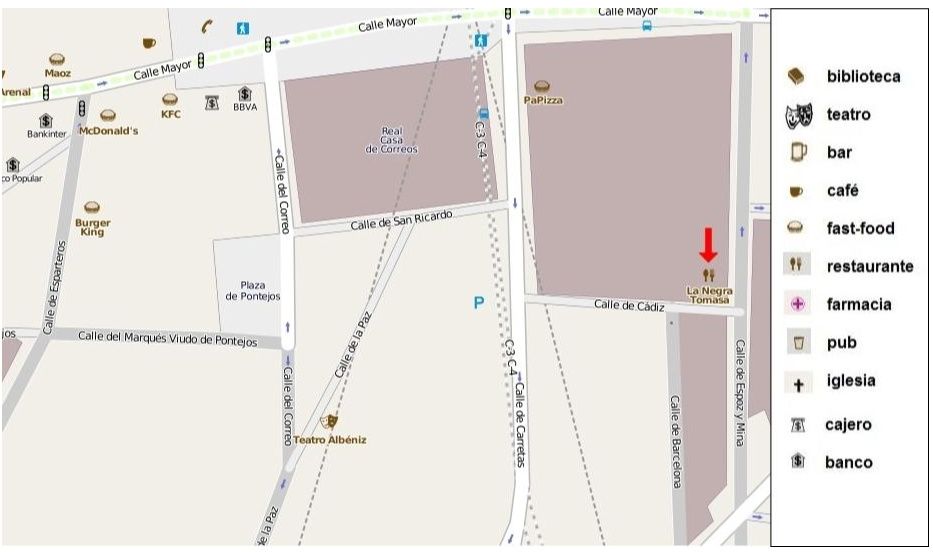
\includegraphics[width=\textwidth]{images/corpus/mapa15.png}
\caption{Fragmento de mapa de la ciudad de Madrid obtenido de OpenStreetMap.}
\label{target_mapa}
\end{figure}

Cuando la informaci\'on del contexto proviene de datos de sensores, las entradas del algoritmo de GER son inevitablemente ruidosas. Es decir, 
contienen informaci\'on no s\'olo incompleta sino tambi\'en posiblemente {\bf incorrecta}. Incluso en contextos tan simples como el de la 
Figura \ref{figura-er} hay incertidumbre: ?`la Tabla \ref{contexto-tabla-propiedades}(b) representa toda la informaci\'on del 
contexto?. Algunos podemos opinar que s\'i, otros que no. En efecto, la persona que gener\'o la ER {\it la pelota a la izquierda del cubo amarillo} opina que no: la relaci\'on \emph{a la izquierda de} entre el target y el cubo amarillo no est\'a representada en la tabla. Un algoritmo de GER con esta tabla como input no puede generar esta expresi\'on referencial. La informaci\'on disponible no s\'olo impide la generaci\'on de ERs v\'alidas, sino que tambi\'en permite la generaci\'on de ERs claramente incorrectas como \emph{la esfera roja 
que no tiene nada a la derecha}.

La tabla puede completarse para que sea posible
generar la expresi\'on referencial. La Figura \ref{representacion-modelo-completo} ilustra una posible forma de completar la informaci\'on de la tabla representada en (a) como un grafo, en el grafo (b). Sin embargo, este nuevo grafo tampoco es completo, 
de hecho, {\it la cosa que est\'a a la derecha del cubo del medio} no se podr\'ia generar con este grafo. Toda representaci\'on de un contexto ser\'a necesariamente incompleta.
%\medskip

\begin{figure}[h]
%\begin{subfigure}{.5\textwidth}
\centering
\vspace*{1cm}
\begin{tabular}{l@{\hspace{1.0cm}}c@{\hspace{1.0cm}}}
\begin{picture}(250,50)
\put(-75,-50){\begin{tikzpicture}
  [
    n/.style={circle,draw,inner sep=1.5pt,node distance=1.5cm},
		 aArrow/.style={->, >=stealth, semithick, shorten <= 1pt, shorten >= 1pt},
  ]
 \node[n,label=below:{
    \relsize{-2}$\begin{array}{c}
      \nSmall\\[-3pt] 
      \nYellow \\[-3pt] 
      \nBall\end{array}$}] (a) {$e_1$};
 \node[n,label=below:{
    \relsize{-2}$\begin{array}{c}     
      \nSmall\\[-3pt] 
      \nRed\\[-3pt] 
      \nCube\end{array}$}, right of=a] (b) {$e_2$};
 \node[n,label=above:{
    \relsize{-2}$\begin{array}{c}     
      \nSmall\\[-3pt] 
      \nYellow\\[-3pt] 
      \nBall\end{array}$}, above of=b] (c) {$e_3$};
 \node[n,label=below:{
    \relsize{-2}$\begin{array}{c}
      \nLarge\\[-3pt] 
      \nRed\\[-3pt] 
      \nCube\end{array}$}, right of=b] (d) {$e_4$};
 \node[n,label=below:{
    \relsize{-2}$\begin{array}{c}
      \nLarge\\[-3pt] 
      \nRed\\[-3pt] 
      \nBall\end{array}$}, right of=d] (e) {$e_5$};
 \node[n,label=below:{
    \relsize{-2}$\begin{array}{c}
      \nSmall\\[-3pt] 
      \nYellow\\[-3pt] 
      \nCube\end{array}$}, right of=e] (f) {$e_6$};
 \node[n,label=below:{
    \relsize{-2}$\begin{array}{c}
      \nSmall\\[-3pt]
      \nRed\\[-3pt] 
      \nCube\end{array}$},  right of=f] (g) {$e_7$};
 \draw [aArrow,bend right=40] (b) to node[auto,swap]{\relsize{-3}$\nBelow$} (c);
 \draw [aArrow,bend right=40] (c) to node[auto,swap]{\relsize{-3}$\nOntop$} (b);
 \draw [aArrow,bend right=40] (d) to node[auto,swap]{\relsize{-3}$\nLeftof$} (e);
 \draw [aArrow,bend right=40] (e) to node[auto,swap]{\relsize{-3}$\nRightof$} (d);
 \draw [aArrow,bend right=40] (f) to node[auto,swap]{\relsize{-3}$\nLeftof$} (g);
 \draw [aArrow,bend right=40] (g) to node[auto,swap]{\relsize{-3}$\nRightof$} (f);
 %\draw[dotted] (-0.5,-1.3) rectangle (8,3.1);
 \draw[dotted] (-0.5,-1.5) rectangle (7.9,3);
 \end{tikzpicture}}
 \end{picture}
 %\end{flushleft}

&
\begin{picture}(50,50)
%\put(172,15){\begin{tikzpicture}
\put(-110,-50){\begin{tikzpicture}
  [    n/.style={circle,draw,inner sep=1.5pt,node distance=1.5cm},
		 aArrow/.style={->, >=stealth, semithick, shorten <= 1pt, shorten >= 1pt},
  ]
 \node[n,label=below:{
    \relsize{-2}$\begin{array}{c}
      \nSmall\\[-3pt] 
      \nYellow \\[-3pt] 
      \nBall\end{array}$}] (a) {$e_1$};
 \node[n,label=below:{
    \relsize{-2}$\begin{array}{c}     
      \nSmall\\[-3pt] 
      \nRed\\[-3pt] 
      \nCube\end{array}$}, right of=a] (b) {$e_2$};
 \node[n,label=above:{
    \relsize{-2}$\begin{array}{c}     
      \nSmall\\[-3pt] 
      \nYellow\\[-3pt] 
      \nBall\end{array}$}, above of=b] (c) {$e_3$};
 \node[n,label=below:{
    \relsize{-2}$\begin{array}{c}
      \nLarge\\[-3pt] 
      \nRed\\[-3pt] 
      \nCube\end{array}$}, right of=b] (d) {$e_4$};
 \node[n,label=below:{
    \relsize{-2}$\begin{array}{c}
      \nLarge\\[-3pt] 
      \nRed\\[-3pt] 
      \nBall\end{array}$}, right of=d] (e) {$e_5$};
 \node[n,label=below:{
    \relsize{-2}$\begin{array}{c}
      \nSmall\\[-3pt] 
      \nYellow\\[-3pt] 
      \nCube\end{array}$}, right of=e] (f) {$e_6$};
 \node[n,label=below:{
    \relsize{-2}$\begin{array}{c}
      \nSmall\\[-3pt]
      \nRed\\[-3pt] 
      \nCube\end{array}$},  right of=f] (g) {$e_7$};
 \draw [aArrow,bend right=40] (b) to node[auto,swap]{\relsize{-3}$\nBelow$} (c);
 \draw [aArrow,bend right=40] (c) to node[auto,swap]{\relsize{-3}$\nOntop$} (b);
 \draw [aArrow,bend right=40] (d) to node[auto,swap]{\relsize{-3}$\nLeftof$} (e);
 \draw [aArrow,bend right=40] (e) to node[auto,swap]{\relsize{-3}$\nRightof$} (d);
 \draw [aArrow,bend right=40] (f) to node[auto,swap]{\relsize{-3}$\nLeftof$} (g);
 \draw [aArrow,bend right=40] (g) to node[auto,swap]{\relsize{-3}$\nRightof$} (f);
 
 \draw [aArrow,bend right=40] (a) to node[auto,swap]{} (b);
 \draw [aArrow,bend right=40] (b) to node[auto,swap]{} (a);

 \draw [aArrow,bend right=40] (b) to node[auto,swap]{} (d);
 \draw [aArrow,bend right=40] (d) to node[auto,swap]{} (b);

\draw [aArrow,bend right=40] (e) to node[auto,swap]{} (f);
 \draw [aArrow,bend right=40] (f) to node[auto,swap]{} (e);
 %\draw[dotted] (-0.5,-1.3) rectangle (8,3.1);
 \draw[dotted] (-0.5,-1.5) rectangle (7.9,3);

 \end{tikzpicture}}

 \end{picture}
%\caption{}
%\end{subfigure}
\vspace{1.8cm}\ \\
        \hspace{1.8cm}(a)&(b)
\end{tabular}
%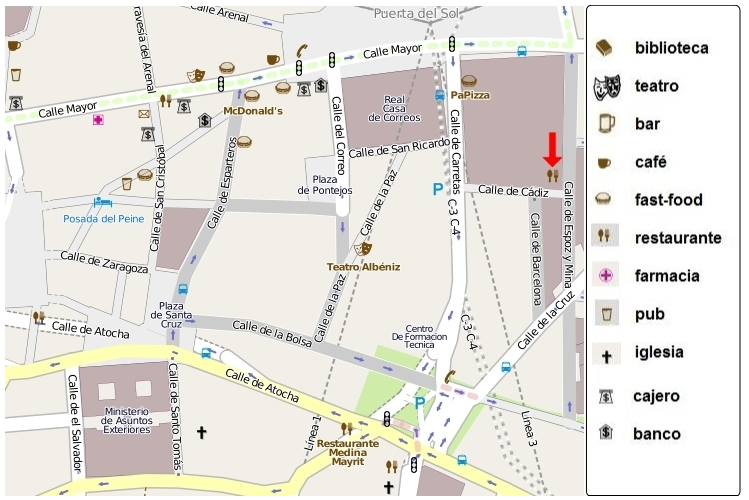
\includegraphics[width=0.46\textwidth]{images/corpus/mapa5.png} & 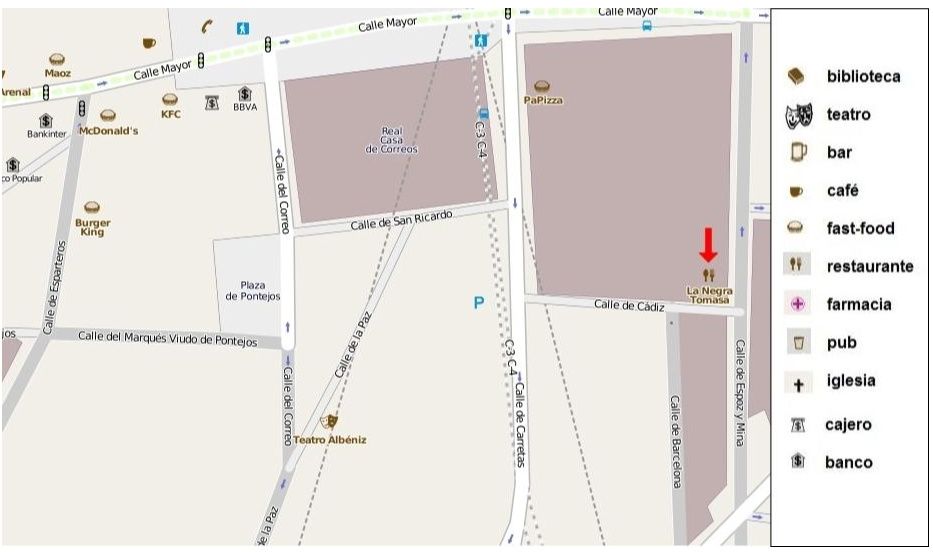
\includegraphics[width=0.53\textwidth]{images/corpus/mapa15.png} \\
%\noindent

\caption{Formalizaci\'on de las propiedades de la Figura \ref{contexto-tabla-propiedades} como un grafo etiquetado en (a) y representaci\'on de contexto m\'as completo en (b).}\label{representacion-modelo-completo}\label{representacion-modelo1}
\end{figure}


Aunque no hablemos ni de incompletitud ni de incorrectitud tambi\'en hay incertidumbre en \textbf{cu\'al} de todas las posibles ERs un sistema de GER debe 
elegir. Por ejemplo seguramente hay personas que preferir\'an ERs que usen la palabra \emph{esfera}, antes que \emph{bola}. Y quiz\'as 
no falte quien diga que \emph{la} mejor expresi\'on referencial para el target ni si quiera aparece en la Figura \ref{figura-er}. Sin embargo, habr\'a una tendencia como se muestra en estudios previos \cite{viet:gene11}: Nadie preferir\'a una ER que use 21 propiedades y 6 relaciones de la tabla para describir al target de la Figura \ref{figura-er}.

El largo de una ER afecta su calidad. Se podr\'{i}a pensar, por ejemplo, que las referencias son \'optimas cuando son \textbf{m\'{i}nimas}
 en longitud, es decir, cuando contienen s\'olo informaci\'on suficiente para identificar el objeto target y nada m\'as. Pero la generaci\'on de referencias m\'{i}nimas
no es lo que las personas hacen ni lo que es m\'as \'util para los oyentes, como se muestra en trabajo previo \cite{Lu_sasha2015,paraboni2007}. Y ni siquiera nos resuelve completamente el problema de elegir una ER: {\it la bola grande} y {\it la esfera roja} son dos ERs de la Figura \ref{figura-er} y tienen 
exactamente la misma longitud.

Dado que la incertidumbre es inherente a la tarea de GER, lo mejor que se puede hacer para ayudar a los sistemas interactivos de GLN es que 
un algoritmo de GER devuelva un \textbf{ranking}
 de ERs, o lo que es lo mismo, un conjunto de ERs en el que cada ER tiene un valor asociado que intenta reflejar cu\'an buena es esa ER para el input dado. Si un sistema interactivo tiene varias ERs para un objeto, puede dar la siguiente frase simplemente seleccionando otra ER, cuando el usuario le indica que no ha entiende la frase. 

?`C\'omo podemos generar un ranking de ERs?.
Un algoritmo simplista generar\'ia primero todas las ERs posibles y luego las ordenar\'ia con alg\'un criterio. Esto es posible porque la cantidad de ERs es finita dado un modelo finito, pero esta cantidad puede ser muy grande, exponencial en el tama\~{n}o del modelo y la gran mayor\'ia de estas ERs no se llegar\'ian a usar en una aplicaci\'on real. Una aplicaci\'on s\'olo usar\'a las mejores ERs de un target considerado.
Una forma m\'as eficiente de generar un ranking de ERs es dise\~{n}ar un algoritmo no determin\'istico que intente generar primero las mejores ERs.

Un algoritmo para GER es {\bf no-determin\'istico} si puede dar diferentes ERs para el mismo contexto y target en sucesivas ejecuciones. 
Para producir un ranking de las mejores ERs para un target, el no determinismo debe estar guiado de alguna forma que le permita preferir ERs mejores y generarlas con una mayor probabilidad. Llamaremos a esta gu\'ia: \textbf{probabilidad de uso} de una propiedad o relaci\'on. Esta probabilidad se puede ver afectada por caracter\'isticas de la propiedad o relaci\'on (algunas propiedades pueden ser m\'as f\'aciles de interpretar que otras) o por caracter\'isticas de qui\'en interpretar\'a la ER (por ejemplo, su conocimiento del idioma).

Hay diferentes \textbf{tipos de propiedades}, por ejemplo taxon\'omicas (las intr\'insecas al objeto target, como \emph{esfera}, o \emph{roja}), relacionales (las que necesitan describir a otro objeto, por ejemplo {\it estar al lado de}), vagas (por ejemplo, \emph{chico}, \emph{grande}, necesitan ser interpretadas con respecto a un contexto, ?`con respecto a qu\'e algo es chico o grande?). Ciertos valores de propiedades pueden ser m\'as f\'aciles de identificar que otros, por ejemplo cierto color verde podr\'{i}a ser m\'as complicado de identificar que el tama\~no grande de un objeto. Notar que cuando decimos el tama\~no, tenemos como marco de referencia a los objetos de la escena, en ese contexto un objeto es {\it grande}.

La selecci\'on de la ER m\'as apropiada tambi\'en debe tener en cuenta al \textbf {interlocutor}, ya que es natural que los humanos demos distintas ERs a distintos interlocutores.
La selecci\'on de qu\'e propiedades y/o relaciones con otros objetos incluir en una expresi\'on referencial depender\'a del prop\'osito que tengamos para dicha expresi\'on referencial. Una expresi\'on referencial ser\'a muy distinta si nuestro objetivo es dar la m\'inima informaci\'on que distinga al objeto, que si nuestro objetivo es ayudar al interlocutor a que identifique el objeto.

La generaci\'on de expresiones referenciales en el mundo real sufre de diversas fuentes de incertidumbre. En esta tesis proponemos formas para modelar esta incertidumbre partiendo de t\'ecnicas de representaci\'on de conocimiento basadas en teor\'ia de modelos y proponiendo como extenderlas usando distribuciones finitas de probabilidades.

\section{Expresiones referenciales usando teor\'ia de modelos}
\label{sec:gre-teoria-modelos}

Los \textbf{modelos relacionales}, tambi\'en conocidos como \textbf{modelos de Kripke} y \textbf{modelos de primer orden}, son muy utilizados para la representaci\'on de situaciones o escenas. 
Los modelos relacionales son grafos etiquetados y pueden verse
tambi\'en como aut\'omatas finitos. Estas estructuras matem\'aticas
han sido muy estudiadas y tienen muchas propiedades bien conocidas
\cite{arec:hybr05b}. 

En esta tesis se adaptan algoritmos cl\'asicos de minimizaci\'on de aut\'omatas aplicados a la caracterizaci\'on de modelos relacionales. Particularmente extendimos t\'ecnicas y algoritmos de teor\'ia de modelos y simulaciones integrando
una distribuci\'on finita de probabilidades que representa esta incertidumbre. Nuestro objetivo
es generar un ranking de las expresiones referenciales ordenado por la probabilidad de ser
correctamente interpretada en el contexto.

Para un \textbf{vocabulario} de s\'imbolos relacionales \emph{r}, un modelo relacional $\+M$ es una tupla $\tup{\Delta,\interp{\cdot}}$ donde:

\begin{itemize}
 \item $\Delta$ es un conjunto no vac\'io de objetos llamado el dominio
 \item $\interp{\cdot}$ es una funci\'on de interpretaci\'on, esto es, $\interp{r} \subseteq \Delta^n$ para todo s\'imbolo de relaci\'on $n$-ario $r$ que est\'a en el vocabulario.  
\end{itemize}

El \textbf{tama\~no} de un modelo $\+M$ es la suma ($\#\Delta + \#\interp{\cdot}$), donde $\#\Delta$ es la cardinalidad
de $\Delta$ y $\#\interp{\cdot}$ es la suma de todas las aridades de las relaciones en $\interp{\cdot}$.
Si asumimos un vocabulario finito de s\'imbolos de relaci\'on $n$-arios, entonces $\+M$ es \emph{finito}. 

A continuaci\'on vamos a presentar 2 ejemplos de modelos relacionales, uno en el que tenemos entidades \textbf{agentivas} (es decir, agentes animados que pueden realizar acciones) como perros y gatos, y otro en el que las entidades son \textbf{no agentivas}, es decir, son objetos est\'aticos.

El primer ejemplo se muestra en la Figura~\ref{grafo-GRE3D7-stimulus_b} donde damos una posible representaci\'on de la escena de la Figura \ref{figura-er} como un modelo relacional. El tama\~no de este modelo es 21, ya que $\#\Delta$=7 y $+\#\interp{\cdot}$=14. 

\begin{figure}[H]
\begin{flushleft}
\begin{tabular}{rcl}
$\Delta$              & = & $\cset{e_1,e_2,e_3,e_4,e_5,e_6,e_7}$\\
$\interp{\aRed}$      & = & $\cset{e_2,e_4,e_5,e_7}$\\
$\interp{\aYellow}$   & = & $\cset{e_1,e_3,e_6}$\\
$\interp{\nBall}$     & = & $\cset{e_1,e_3,e_5}$\\
$\interp{\nCube}$     & = & $\cset{e_2,e_4,e_6,e_7}$\\

$\interp{\aSmall}$    & = & $\cset{e_1,e_2,e_3,e_6,e_7}$\\
$\interp{\aLarge}$    & = & $\cset{e_4,e_5}$\\

$\interp{\nLeftof}$   & = & $\cset{(e_4,e_5),(e_6,e_7)}$\\
$\interp{\nRightof}$    & = & $\cset{(e_5,e_4),(e_7,e_6)}$\\
$\interp{\nOntop}$     & = & $\cset{(e_3,e_2)}$\\
$\interp{\nBelow}$     & = & $\cset{(e_2,e_3)}$\\

 \end{tabular}
\begin{picture}(120,50)
\put(0,-50){\begin{tikzpicture}
  [
    n/.style={circle,draw,inner sep=1.5pt,node distance=1.5cm},
		 aArrow/.style={->, >=stealth, semithick, shorten <= 1pt, shorten >= 1pt},
    %aSniffing/.style={->, >=stealth, semithick, shorten <= 3pt, shorten >= 3pt},
  ]
%\begin{tikzpicture}
%  [
%    n/.style={circle,fill,draw,inner sep=3pt,node distance=2cm},
%    aArrow/.style={->, >=stealth, semithick, shorten <= 1pt, shorten >= 1pt},
%  ]
 \node[n,label=below:{
    \relsize{-2}$\begin{array}{c}
      \nSmall\\[-3pt] 
      \nYellow \\[-3pt] 
      \nBall\end{array}$}] (a) {$e_1$};
 \node[n,label=below:{
    \relsize{-2}$\begin{array}{c}     
      \nSmall\\[-3pt] 
      \nRed\\[-3pt] 
      \nCube\end{array}$}, right of=a] (b) {$e_2$};
 \node[n,,label=above:{
    \relsize{-2}$\begin{array}{c}
      \nSmall\\[-3pt] 
      \nYellow\\[-3pt] 
      \nBall\end{array}$}, above of=b] (c) {$e_3$};
 \node[n,label=below:{
    \relsize{-2}$\begin{array}{c}
      \nLarge\\[-3pt] 
      \nRed\\[-3pt] 
      \nCube\end{array}$}, right of=b] (d) {$e_4$};
 \node[n,label=below:{
    \relsize{-2}$\begin{array}{c}
      \nLarge\\[-3pt] 
      \nRed\\[-3pt] 
      \nBall\end{array}$}, right of=d] (e) {$e_5$};
 \node[n,,label=below:{
    \relsize{-2}$\begin{array}{c}
      \nSmall\\[-3pt] 
      \nYellow\\[-3pt] 
      \nCube\end{array}$}, right of=e] (f) {$e_6$};
 \node[n,label=below:{
    \relsize{-2}$\begin{array}{c}
      \nSmall\\[-3pt]
      \nRed\\[-3pt] 
      \nCube\end{array}$},  right of=f] (g) {$e_7$};
 \draw [aArrow,bend right=40] (b) to node[auto,swap]{\relsize{-3}$\nBelow$} (c);
 \draw [aArrow,bend right=40] (c) to node[auto,swap]{\relsize{-3}$\nOntop$} (b);
 \draw [aArrow,bend right=40] (d) to node[auto,swap]{\relsize{-3}$\nLeftof$} (e);
 \draw [aArrow,bend right=40] (e) to node[auto,swap]{\relsize{-3}$\nRightof$} (d);
 \draw [aArrow,bend right=40] (f) to node[auto,swap]{\relsize{-3}$\nLeftof$} (g);
 \draw [aArrow,bend right=40] (g) to node[auto,swap]{\relsize{-3}$\nRightof$} (f);
 
%\draw[dotted] (-0.5,-1.3) rectangle (8,3.1);

% \end{tikzpicture}
%\caption{Grafo del contexto \ref{GRE3D7-stimulus}}
%\label{grafo-GRE3D7-stimulus_b}
%\end{figure}
 \end{tikzpicture}}
 \end{picture}
 \end{flushleft}
 \caption{Representaci\'on de la escena de la Figura \ref{figura-er} como un modelo relacional e interpretaci\'on de sus propiedades y relaciones. Ejemplo con entidades no agentivas.}
 \label{grafo-GRE3D7-stimulus_b}
 \end{figure}
 
El dominio es $\Delta$  = $\cset{e_1,e_2,e_3,e_4,e_5,e_6,e_7}$. La interpretaci\'on de $\nBall$ es $e_1$, $e_3$ y $e_5$, ya que estos objetos son esferas, la de $\nCube$ es $\interp{\nCube}$ = $\cset{e_2, e_4, e_6, e_7}$, ya que esos objetos son cubos. Tenemos las relaciones $\nRightof$, $\nLeftof$, $\nBelow$ y $\nOntop$, cuyas interpretaciones se muestran en la figura. Como discutimos en la secci\'on anterior, se puede argumentar que este modelo est\'a incompleto, pero es suficiente para los objetivos ilustrativos de esta secci\'on.

El segundo ejemplo se muestra en la Figura~\ref{fig:cat-dog-1} en la cual hemos representado un contexto agentivo como un modelo relacional. En el modelo, $a$, $b$ y $d$ son perros, mientras que 
$c$ y $e$ son gatos;  $d$ es un peque\~no beagle; $b$ y $c$ tambi\'en son peque\~nos.
 Leeremos $\aSniffing(d,e)$ como ``{\em $d$ huele a $e$}''. La interpretaci\'on del s\'imbolo relacional $\nDog$ es $\interp{\nDog}$  =  $\cset{a,b,d}$ ya que $a$, $b$ y $d$ son los \'unicos perros del contexto. La interpretaci\'on de $\aSniffing$ es el conjunto de pares de elementos que cumplen $\aSniffing$. Por ejemplo ($a,a$) pertenece al conjunto dado que $a$ es un perro que se huele a s\'i mismo en el modelo. El tama\~no de este modelo es 11, ya que $\#\Delta$=5 y $+\#\interp{\cdot}$=6. 

 \begin{figure}[H]
 %\begin{center}
 \begin{tabular}{rcl}
$\Delta$               & = & $\cset{a,b,c,d,e}$\\
$\interp{\nDog}$      & = & $\cset{a,b,d}$\\
$\interp{\nCat}$      & = & $\cset{c,e}$\\
$\interp{\nBreed}$    & = & $\cset{d}$\\
$\interp{\aSmall}$    & = & $\cset{b,c,d}$\\
$\interp{\aSniffing}$ & = & $\cset{(a,a),(b,a),(c,b),(d,e),(e,d)}$
 \end{tabular}
\begin{picture}(90,30)
\put(0,-40){\begin{tikzpicture}
  [
    n/.style={circle,draw,inner sep=1.5pt,node distance=1.5cm},
    aSniffing/.style={->, >=stealth, semithick, shorten <= 3pt, shorten >= 3pt},
  ]
 \node[n,label=below:{\relsize{-1}$\begin{array}{c}\nDog\end{array}$}] (a) {$a$};

 \node[n,label=below:{\relsize{-1}$\begin{array}{c}\nDog\\ \aSmall \end{array}$}, right of=a] (b) {$b$};

 \node[n,label=below:{\relsize{-1}$\begin{array}{c}\nCat\\ \aSmall\end{array}$}, right of=b] (c) {$c$};

 \node[n,label=below:{\relsize{-1}$\begin{array}{c}\nDog\\ \nBreed\\  \aSmall \end{array}$}, right of=c] (d) {$d$};

 \node[n,label=below:{\relsize{-1}$\begin{array}{c}\nCat\end{array}$},right of=d] (e) {$e$};

 \draw [aSniffing,loop left] (a) to node[above,xshift=-5pt]{\relsize{-1}$\aSniffing$} (a);

 \draw [aSniffing,bend right=40] (b) to node[auto,swap]{\relsize{-1}$\aSniffing$} (a);

 \draw [aSniffing,bend right=40] (c) to node[auto,swap]{\relsize{-1}$\aSniffing$} (b);

 \draw[aSniffing, bend left=40] (d) to node[auto]{\relsize{-1}$\aSniffing$} (e);
 \draw[aSniffing, bend left=40] (e) to node[auto,swap]{\relsize{-1}$\aSniffing$} (d);

 \end{tikzpicture}}
 \end{picture}

 %\end{center}
 \caption{Representaci\'on de un contexto agentivo como un modelo relacional e interpretaci\'on de sus propiedades y relaciones.\label{fig:cat-dog-1}}
 \end{figure}

Ahora nos enfocaremos en conseguir ERs para identificar a targets dados usando los modelos que acabamos de describir. Veremos lenguajes de distintas l\'ogicas y c\'omo las f\'ormulas l\'ogicas pueden representar a las ERs.
A continuaci\'on definimos el lenguaje cl\'asico de la l\'ogica de primer orden (con desigualdad), \FOL. Dicho lenguaje se define inductivamente como sigue. \\
Una f\'ormula $\phi$ es una f\'ormula de \FOL si es de alguna de las siguientes formas:


\medskip

\begin{enumerate}
  \item $\top$ es como decir {\it cosa} o \emph{ese}, todo elemento del modelo satisface $\top$.
  \item $x_i \not\approx x_j$ La desigualdad entre dos elementos $x_i$ y $x_j$.
  \item $r (\bar x)$ Relaciones de tuplas.
  \item $\lnot \gamma$ Negaci\'on de f\'ormulas.
  \item $\gamma \land \gamma'$ Conjunci\'on de f\'ormulas.
  \item $\exists x_i . \gamma$ Existencial de una variable ligada en la f\'ormula $\gamma$.
\end{enumerate}
%
donde $\gamma,\gamma' \in \FOL$,
$r$ es un s\'imbolo de relaci\'on $n$-aria y $\bar x$ es una tupla de $n$ variables.
Como es usual, $\gamma \lor \gamma'$ y $\forall x . \gamma$ son las versiones cortas de
$\lnot(\lnot\gamma \land \lnot\gamma')$ y $\lnot\exists x . \lnot\gamma$, respectivamente.
F\'ormulas de la forma $\top$, $x_i \not\approx x_j$ y $r(\bar
x)$ son llamadas \emph{\'atomos}.%

Dado un modelo relacional $\+M = \tup{\Delta,\interp{\cdot}}$ y una
f\'ormula $\gamma$ con variables libres%
\footnote{%
    Asumimos que cada variable no puede aparecer libre y ligada a la vez, que una variable no est\'a ligada 2 veces,
    y que el \'indice de las variables crece en la f\'ormula de izquierda a derecha.%
}
$x_1\ldots x_n$, inductivamente definimos la \textbf{extensi\'on} o
\textbf{interpretaci\'on} de $\gamma$ como el conjunto de $n$-tuplas
 $\interp{\gamma}^n \subseteq \Delta^n$ que satisface:

\begin{enumerate}

\item $\interp{\top}^n$ $=$ $\Delta^n$

\item $\interp{x_i \not\approx x_j}^n$ $=$ $\cset{\bar{a} \mid \bar{a} \,{\in}\, \Delta^n, a_i \neq a_j}$

\item $\interp{\lnot\delta}^n$ $=$ $\Delta^n \setminus \interp{\delta}^n$

\item $\interp{r (x_{i_1} \ldots x_{i_k})}^n$ $=$ $\cset{\bar{a} \mid \bar{a} \,{\in}\, \Delta^n, (a_{i_1} \ldots a_{i_k}) {\in} \interp{r}}$

\item $\interp{\delta \land \theta}^n$ $=$ $\interp{\delta}^n \cap \interp{\theta}^n$

\item $\interp{\exists x_{l}.\delta}^n$ $=$ $\cset{\bar a \mid \bar a  e  \in \interp{\delta'}^{n+1}\ \text{para alg\'un elemento $e$}}$

\end{enumerate}

donde $1 \le i,j, i_1, \ldots, i_k \le n$, $\bar{a} = (a_1\ldots
a_n)$, $\bar{a}e = (a_1\ldots a_n,e)$ y $\delta'$ son
obtenidos reemplazando todas las ocurrencias de $x_l$ en $\delta$ por
$x_{n+1}$. 
%Cuando la cardinalidad de las tuplas involucradas en el contexto es conocida 
%escribiremos $\interp{\phi}$ en lugar de
%$\interp{\phi}^n$.

Con una sintaxis y sem\'antica de un lenguaje en mente, podemos formalmente definir el problema de \textbf{GER en $\gL$} ($\gL$-GER) para un conjunto target $T$ de elementos. $\gL$ es el lenguaje de la l\'ogica elegida, en este caso hemos explicado la l\'ogica de primer orden $\FOL$, y en el Cap\'itulo \ref{sec:intro_logica} restringiremos esa l\'ogica para obtener ERs m\'as cercanas a las que aparecen en corpora y para conseguir algoritmos computacionalmente m\'as eficientes.

\medskip
\noindent
{\small
\begin{center}
\begin{tabular}{ll} \hline
\multicolumn{2}{l}{
\textsc{Problema $\gL$-GER }}\\ \hline
\ \ Entrada: & un modelo $\gM=\tup{\Delta,\interp{\cdot}}$ y un conjunto target no vac\'io $T \subseteq \Delta$.\\
\ \ Salida: & una f\'ormula $\varphi \in \gL$ tal que
$\interp{\varphi} = T$ si existe, y $\bot$ caso contrario.\\ \hline
\end{tabular}
\end{center}}
\medskip
La salida del problema $\+L$-GER es una f\'ormula de
$\+L$ cuya interpretaci\'on en el modelo de input $\gM$ es el conjunto target $T$, si
esa f\'ormula existe. 
Cuando la salida no es $\bot$, decimos que $\phi$ es una
\textbf{expresi\'on referencial en $\+L$ (ER-$\+L$)} para $T$ en $\+M$, y cuando es $\bot$ puede ser que la l\'ogica elegida no sea lo suficientemente expresiva para identificar al target, o que el modelo dado no tenga suficiente detalle.

Consideramos s\'olo modelos relacionales con s\'imbolos de relaciones unarias y binarias, usaremos $p$ para las proposiciones (propiedades) y $r$ para los s\'imbolos de relaci\'on binarias.
Como dijimos anteriormente, dado un modelo $\gM$, podr\'ia haber un n\'umero muy grande de f\'ormulas que de forma un\'ivoca
describan al target (incluso f\'ormulas que no son l\'ogicamente equivalentes podr\'ian tener
la misma interpretaci\'on una vez que el modelo este fijo). Por ejemplo, en el modelo $\+M$ de la Figura \ref{grafo-GRE3D7-stimulus_b} las f\'ormulas $\aLarge \land \nBall$ y $\aRed \land \nBall$ no son l\'ogicamente equivalentes pero tienen la misma interpretaci\'on en $\gM$ ya que $\interp{\aLarge \land \nBall}$ = \{$e_5$\} y $\interp{\aRed \land \nBall}$ = \{$e_5$\}. Diferentes ERs del mismo target podr\'ian ser m\'as o menos apropiadas en el contexto dado. Otra cosa que es importante tener en cuenta, es que la determinaci\'on de contenido usando lenguajes con diferente poder expresivo, puede tener un impacto en la complejidad computacional de la GER y en la etapa posterior de realizaci\'on sint\'actica. Para ilustrar eso, veamos las f\'ormulas que identifican al elemento target $b$ en la Figura \ref{fig:cat-dog-1}.
\medskip
$$
\begin{array}{ll}
 \phi_1:  \nDog(x) \land \aSmall(x) \land
   \exists y . (\aSniffing(x,y) \land \nDog(y))\\
  %
  \phi_2:  \nDog(x) \land \aSmall(x) \land
  \forall y . (\neg \nCat(y) \lor \neg \aSniffing(x,y))\\
  %
  \phi_3:  \nDog(x) \land
  \exists y . (x \not\approx y \land \nDog(y)  \land \aSniffing(x,y))\\
  %
  \phi_4:  \nDog(x) \land
  \exists y . (\nCat(y) \land \aSmall(y) \land \aSniffing(y,x))
  %
 \end{array}
$$

Notar que las f\'ormulas mostradas, hacen uso de diferentes operadores de la l\'ogica \FOL: hay negaci\'on de \'atomos y de relaciones, hay cuantificaci\'on existencial, y universal, conjunci\'on, disyunci\'on y desigualdad. La realizaci\'on sint\'actica de algunas de \'estas f\'ormulas pueden involucrar estructuras gramaticales complejas. Por ejemplo la f\'ormula $\phi_4$ requiere el uso de voz pasiva y podr\'ia realizarse como {\it el perro que es olido por un gato peque\~no}. La f\'ormula $\nDog(x) \land \exists y . (x \not\approx y \land \nDog(y) \land \aSniffing(x,y))$ que representa al target $b$ de la Figura \ref{fig:cat-dog-1} requiere el uso de lexemas como otro y puede realizarse como {\it el perro que huele a otro perro}. La f\'ormula $\phi_2$ requiere el uso de negaci\'on del predicado y podr\'ia realizarse como {\it el perro peque\~no que no huele gatos}.
 
Como nuestra meta es hacer un ranking de las mejores expresiones referenciales, una manera de acercarnos a esa meta es restringiendo la l\'ogica. Si restringimos a \EPFOL que no tiene negaci\'on, aseguramos que f\'ormulas como $\phi_2$ no se generar\'an. Si sac\'aramos el operador distinto ($\not\approx$) del lenguaje, $\phi_3$ tambi\'en queda excluida.
A continuaci\'on presentamos fragmentos de $\FOL$ conocidos como l\'ogicas de descripci\'on. Por ejemplo, el lenguaje de la l\'ogica de descripci\'on $\ALC$ de \cite{arec:hybr05b}, se define sint\'acticamente como el conjunto de f\'ormulas que se pueden generar recursivamente como sigue
$$
\top \mid p \mid \neg \phi \mid \phi \wedge \phi' \mid  \exists r. \phi
$$
donde $p$ es un s\'imbolo proposicional, $r$ es un s\'imbolo relacional binario, y $\phi$, $\phi'$ son f\'ormulas de $\ALC$.

 Mediante la restricci\'on a f\'ormulas de $\ALC$ 
evitar\'iamos f\'ormulas como $\phi_3$ (es decir con desigualdad). Tambi\'en evitar\'iamos f\'ormulas como $\phi_4$ ({\it el perro que es olido por un peque\~no gato}) en la cual tenemos que realizar la parte del existencial como una voz pasiva al aparecer la variable $x$ en segundo lugar.

Cada lenguaje l\'ogico puede ser visto como un compromiso entre la expresividad, realizabilidad y complejidad computacional. Para la tarea de GER el uso de un lenguaje u otro debe depender del contexto particular considerado y del target a describir.

Para el segundo ejemplo, supongamos que queremos identificar al objeto $e_5$ de la Figura \ref{grafo-GRE3D7-stimulus_b}. Algunas f\'ormulas posibles  que identifican un\'ivocamente a $e_5$ en el modelo se muestran a continuaci\'on.
$$
\begin{array}{ll}
 \phi_1: & \aRed(x) \land \nBall(x)\\[2pt]
  %
 \phi_2: & \aLarge(x) \land \nBall(x)\\[2pt]
  %
 \phi_3: & \nLarge(x) \land \aRed(x) \land \nBall(x)\\[2pt]
  %
 \phi_4: & \nLarge(x) \land \aRed(x) \land \nBall(x) \land
   \exists y . (\nRightof(x,y) \land \aLarge(y) \land \aRed(y) \land \nCube(y))\\[2pt]
  %ex1
 \phi_5: & \nLarge(x) \land \aRed(x) \land \nBall(x) \land
  \forall y . (\neg \nBall(y) \lor \neg \nRightof(x,y))\\[2pt]
  %ex 2
 \phi_6: & \nLarge(x) \land \aRed(x) \land \nBall(x) \land
  \exists y . (x \not\approx y \land \nCube(y) \land \nRightof(x,y))\\[2pt]
  %ex 3
 \phi_7: & \nLarge(x) \land \aRed(x) \land \nBall(x) \land
  \exists y . (\nCube(y) \land \aRed(y) \land \nLeftof(y,x))
  %ex 4
 \end{array}
$$
Las f\'ormulas que no contienen negaci\'on se pueden representar como subgrafos como se muestran en la Figura \ref{grafos-formulas}. El de la izquierda representa la f\'ormula $\phi_1$ y el de la derecha a la f\'ormula $\phi_4$.

 \begin{figure}[h]
 %\begin{center}
%\hspace*{1.5cm} 
\begin{picture}(0,60)
\put(140,0){\begin{tikzpicture}
  [
    n/.style={circle,draw,inner sep=1.5pt,node distance=1.5cm},
		 aArrow/.style={->, >=stealth, semithick, shorten <= 1pt, shorten >= 1pt},
  ]
 \node[n,label=below:{
    \relsize{-2}$\begin{array}{c}
      \nRed\\[-3pt] 
      \nBall\end{array}$}, right of=d] (e) {$e_5$};
 \end{tikzpicture}}
\end{picture}
\begin{picture}(0,70)
%\hspace*{3.5cm} 
%\vspace*{5.5cm} 

\put(250,-8){\begin{tikzpicture}
   [
    n/.style={circle,draw,inner sep=1.5pt,node distance=1.5cm},
		 aArrow/.style={->, >=stealth, semithick, shorten <= 1pt, shorten >= 1pt},
  ]
 \node[n,label=below:{
    \relsize{-2}$\begin{array}{c}
      \nLarge\\[-3pt] 
		  \nRed\\[-3pt] 
      \nCube\end{array}$}, right of=b] (d) {$e_4$};
 \node[n,label=below:{
    \relsize{-2}$\begin{array}{c}
      \nLarge\\[-3pt]
      \nRed\\[-3pt] 
      \nBall\end{array}$}, right of=d] (e) {$e_5$};
 \draw [aArrow,bend right=40] (e) to node[auto,swap]{\relsize{-3}$\nRightof$} (d);
 \end{tikzpicture}}
 \end{picture}
%\end{subfigure}
\caption{Subgrafos que representan las f\'ormulas $\phi_1$ y $\phi_4$.}\label{grafos-formulas}
%\end{center}
\end{figure}


Las f\'ormulas $\phi_1$ a $\phi_7$ pueden realizarse como sigue.
\smallskip

\begin{tabular}{l}
 $\phi_1$: {\it La esfera roja}\\[1pt]
  %
 $\phi_2$: {\it La esfera grande}\\[1pt]
  %
 $\phi_3$: {\it La esfera grande y roja}\\[1pt]
  %
 $\phi_4$: {\it La esfera grande y roja que est\'a a la derecha de un cubo grande y rojo}\\[1pt]
  %ex1
 $\phi_5$: {\it La esfera grande y roja, que no tiene ninguna esfera a la derecha}\\[1pt]
  %ex 2
 $\phi_6$: {\it La esfera grande y roja que est\'a a la derecha de un cubo}\\[1pt]
 % (x \not\approx y \land \nCube(y) \land \nRightof(x,y))
  %ex 3
 $\phi_7$: {\it La esfera grande y roja que tiene un cubo rojo a la izquierda}\\[1pt]
  %ex 4
\end{tabular}
%%$$
\smallskip

Notar que $\phi_1$ y $\phi_2$ son m\'inimas, es decir no se puede dar una f\'ormula m\'as corta que esas que identifique al target.
Las f\'ormulas $\phi_1$, $\phi_2$, $\phi_3$, $\phi_4$ y $\phi_6$ son caracterizadas como f\'ormulas positivas, conjuntivas y existenciales (no contienen negaci\'on y s\'olo tienen conjunciones, cuantificadores existenciales y desigualdad), este tipo de f\'ormulas son las que m\'as se encuentran en corpora de ERs~\cite{viethen06:_algor_for_gener_refer_expres,deemter06:_build_seman_trans_corpus_for,gre3d3}. Luego como dijimos reci\'en, podemos elegir otra l\'ogica cuyo lenguaje est\'e restringido a las ERs que queremos generar. Restringiendo la determinaci\'on de contenido a \EPFOL, aseguramos que f\'ormulas como  $\phi_5$ no se generar\'an. Si prohibimos el distinto del lenguaje, $\phi_6$ tambi\'en queda excluida. La l\'ogica de menor complejidad computacional que se corresponde con todas esas restricciones es \EL, la cual est\'a dada por:
$$
\top \mid p \mid \gamma \wedge \gamma' \mid  \exists r. \gamma
$$
donde $p$ es un s\'imbolo proposicional, $r$ un s\'imbolo de relaci\'on binaria, y $\gamma,\gamma' \in \EL$, es decir son f\'ormulas de $\EL$. $\EL$ se corresponde con el fragmento
 de \ALC sin negaci\'on.

En el Cap\'itulo \ref{sec:intro_logica} describimos c\'omo los operadores l\'ogicos afectan la expresividad y la complejidad computacional de la tarea de GER, as\'i como las ERs generadas. En el Cap\'itulo \ref{sec:algoritmo} proponemos como generar no una sino un ranking de ERs y agregamos una distribuci\'on finita de probabilidades asociada a los s\'imbolos de relaci\'on del modelo.



\section{Mapa de la tesis}
\label{sec:mapadetesis}

En esta secci\'on contamos como est\'a organizada la tesis. En lo que sigue daremos el resumen de la tem\'atica de cada cap\'itulo.

\subsection{Cap\'itulo~\ref{sec:intro}: ``Introducci\'on''} 
Situamos a la generaci\'on autom\'atica de expresiones 
referenciales dentro de la inteligencia artificial y de la generaci\'on de lenguaje natural. Dijimos que un sistema de 
generaci\'on de lenguaje natural tiene tres etapas: la determinaci\'on de contenido, la lexicalizaci\'on y la realizaci\'on sint\'actica. La generaci\'on de expresiones referenciales es una sub\'area de la generaci\'on de lenguaje natural y por lo tanto, incluye las mismas tres etapas. La determinaci\'on de contenido, que es la selecci\'on de las propiedades y/o relaciones con otros objetos que vamos a elegir para identificar un\'ivocamente al target, es el tema de la tesis. Explicamos conceptos b\'asicos que usamos a lo largo de la tesis, como {\it dominio}, {\it contexto}, {\it propiedad}, {\it target}, {\it distractor} y {\it algoritmo}. Explicamos porqu\'e la tarea de GER es compleja, ya que hay incertidumbre al representar el contexto en situaciones de la vida real. Los modelos son indefectiblemente incompletos o incorrectos. Dimos una introducci\'on a la variedad de expresiones referenciales que 
se puede tener para el mismo objeto target en el mismo contexto. Propusimos dar no una ER sino un ranking de ERs para un input dado.
Introdujimos el concepto de teor\'ia de modelos, describimos diversos lenguajes formales (es decir, l\'ogicos) y su impacto al ser usados en el problema de generaci\'on autom\'atica de expresiones referenciales.  Partimos desde la l\'ogica de primer orden (\FOL), la m\'as expresiva, explicamos el lenguaje asociado, para darnos una idea de cu\'ales son las f\'ormulas que el lenguaje puede generar, vimos una serie de ejemplos y propusimos restricciones al lenguaje que permiten generar estructuras que se ven en corpora.

\subsection{Cap\'itulo~\ref{sec:seleccion}: ``Generaci\'on de expresiones referenciales''} 
Este cap\'itulo est\'a dividido en 4 secciones. En la primer secci\'on definimos los diferentes tipos de expresiones referenciales: proposicionales, relacionales, minimales, sobreespecificadas, subespecificadas. Luego comentamos en qu\'e se basan la teor\'ia introducida en \cite{clark1992arenas,clark96,Clark-Marshall81} y c\'omo son refutadas por algunas investigaciones. Mostramos informaci\'on b\'asica de corpora existente en el \'area, varios de los cuales usaremos a lo largo de la tesis. Viendo la simplicidad de estos corpora, por un lado podemos ver la complejidad de la tarea, ya que si para corpora tan simples, es tan dif\'icil conseguir algoritmos que hagan lo que hacen los humanos, podr\'iamos imaginarnos que es realmente una tarea mucho m\'as dif\'icil en contextos que la gente usa en la vida diaria. Por otro lado, motivamos la obtenci\'on de un nuevo corpus, el cual describimos en el Cap\'itulo \ref{sec:corpus}, que usa im\'agenes de mapas de ciudades como contextos. En la segunda secci\'on describimos diferentes tipos de algoritmos para la tarea de generaci\'on autom\'atica de expresiones referenciales: determin\'isticos, no-determin\'isticos, que generan sobreespecificaci\'on, plurales, s\'olo singulares, relacionales o proposicionales. Se estudi\'o el avance en el \'area de la generaci\'on autom\'atica de expresiones referenciales, los algoritmos existentes, se compararon esos algoritmos en cuanto al tipo de algoritmo y salida que producen. Se explica el algoritmo Graph en m\'as detalle que los dem\'as porque es el m\'as cercano a los tipos de algoritmos que se extienden en esta tesis. Luego en la tercer secci\'on damos una introducci\'on a las m\'etricas de evaluaci\'on de la tarea de GER. Algunas m\'etricas usan corpus para comparar las salidas de los algoritmos con las ERs dadas por humanos. Hay m\'etricas autom\'aticas y otras manuales. Para finalizar el cap\'itulo damos un resumen y explicamos c\'omo se linkea con los dem\'as cap\'itulos.

\subsection{Cap\'itulo~\ref{sec:intro_logica}: ``Usando teor\'ia de modelos''} 
Damos definiciones b\'asicas de modelo, interpretaci\'on y f\'ormula. Explicamos de la noci\'on de similaridad de 2 elementos $u$ y $v$ del modelo la cual dice que son similares en $\+L$, cuando para toda f\'ormula $\phi \in \+L$, tenemos que 
$\{u,v\} \subseteq \interp{\phi}$. Se dice que $u$ y $v$ son indistinguibles en el lenguaje l\'ogico $\+L$, ya que no hay una f\'ormula que satisfaga uno y no el otro. El concepto de \emph{similaridad} puede ser usado para definir la tarea GER pero implica generar posiblemente infinitas f\'ormulas. Veremos que para modelos finitos la $\+L$-similaridad puede definirse en t\'erminos de $\+L$-simulaciones lo cual nos permitir\'a saber si hay una ER para el target sin checkear infinitas f\'ormulas. Se adaptan algoritmos conocidos de simulaci\'on para varias l\'ogicas tales como \ALC y \EL entre otras para la GER. Explicamos c\'omo computamos las ERs para los distintos lenguajes l\'ogicos \EPFOL, \ALC y \EL. Clasificamos los algoritmos vistos seg\'un la complejidad computacional de los mismos. 

\subsection{Cap\'itulo~\ref{sec:algoritmo}: ``Modelando la incertidumbre''} 
En este cap\'itulo 
explicamos nuestra propuesta de agregar probabilidades de uso a las palabras de la signatura del modelo para representar la incertidumbre del contexto, adaptando algoritmos introducidos en el Cap\'itulo \ref{sec:intro_logica}. Mostramos que los algoritmos permiten sobreespecificaci\'on, 
pero aseguran terminaci\'on y agregamos un componente aleatorio para conseguir no-determinismo y as\'i generar un ranking de ERs. Mostramos en detalle el input que toma el
 nuevo algoritmo. Explicamos c\'omo obtener las probabilidades de uso que toma como input el algoritmo a partir de corpus usando aprendizaje autom\'atico. Para la tarea de aprendizaje autom\'atico usamos caracter\'isticas independientes del dominio. 
Mostramos la salida del algoritmo, explicamos c\'omo conseguimos no-determinismo en las distintas ejecuciones del algoritmo y c\'omo aseguramos 
terminaci\'on. Adem\'as mostramos completitud, es decir que siempre conseguimos una expresi\'on referencial si existe. Explicamos c\'omo agregamos sobreespecificaci\'on a las expresiones referenciales. Finalmente mostramos un ejemplo de ejecuci\'on. 

\subsection{Cap\'itulo~\ref{sec:evaluacion}: ``Evaluaci\'on de rankings sobre benchmarks''} 
En el Cap\'itulo \ref{sec:seleccion} se describieron m\'etricas de evaluaci\'on tanto autom\'aticas como manuales. Evaluamos los algoritmos presentados 
en el Cap\'itulo \ref{sec:algoritmo}, teniendo en cuenta ambos tipos de m\'etricas. La evaluaci\'on est\'a dividida en 2 partes. 
Una parte en la cual comparamos la salida del algoritmo para modelos de 2 corpora descriptos en el Cap\'itulo \ref{sec:seleccion}, con expresiones referenciales dadas por los humanos, tomando como input probabilidades de uso obtenidas con aprendizaje autom\'atico a partir de cada corpora. Vemos c\'omo las ERs generadas con probabilidades obtenidas del corpus con aprendizaje autom\'atico se acercan 
mucho m\'as a las humanas, que 2 baselines (random y uniforme). En la otra parte de este cap\'itulo presentamos una evaluaci\'on manual en la cual 2 jueces humanos decidieron qu\'e ER era mejor entre la del corpus y la generada por el algoritmo. Es interesante notar c\'omo muchas 
veces las ERs generadas por el algoritmo fueron juzgadas por los jueces como mejores que las humanas. El algoritmo tiene la ventaja de que
 siempre da una ER si existe, en cambio los humanos muchas veces dan expresiones ambiguas que no son referenciales. 

\subsection{Cap\'itulo~\ref{sec:corpus}: ``Recolecci\'on y an\'alisis del corpus ZOOM''} Introducimos un nuevo corpus, 
el ZOOM corpus, el cual fue recolectado en un trabajo conjunto con la Universidad de S\~ao Paulo (Brasil), 
para tener un corpus de un dominio m\'as natural de expresiones referenciales. El corpus ZOOM contiene expresiones referenciales 
de puntos de inter\'es en mapas. Los mapas son fragmentos de las ciudades de Madrid y Lisboa. Este corpus fue recolectado en 2 idiomas, 
espa\~nol y portugu\'es. Contiene todos los tipos de ERs presentados en el Cap\'itulo \ref{sec:seleccion}. Se explica el m\'etodo de recolecci\'on del corpus, se dan estad\'isticas de las personas que completaron el 
experimento y se explica la manera en que se anot\'o el corpus. Se describe brevemente y se eval\'ua sobre este corpus un m\'etodo puramente basado en aprendizaje autom\'atico que usa {\it support vector machines}, para decidir si incluir o no una propiedad en la ER de salida. Adem\'as se eval\'ua el desempe\~no de nuestros algoritmos sobre un fragmento del corpus ZOOM.

\subsection{Cap\'itulo~\ref{sec:conclusiones}: ``Conclusiones y trabajo futuro''} En este cap\'itulo se da un resumen de lo estudiado, se explican los avances realizados en esta tesis, como la incorporaci\'on de distribuciones finitas de probabilidades a algoritmos determin\'isticos que usan simulaciones para la GER. Esta distribuci\'on de probabilidades la aprendemos desde corpora con funciones de regresi\'on lineal. Los algoritmos est\'an inspirados en el modelo psicoling\"u\'istico de GER que determina la forma de sobreespecificar. Evaluamos los rankings obtenidos con una serie de benchmarks del \'area usando m\'etricas autom\'aticas y humanas. Creamos un nuevo corpus de ERs, el ZOOM corpus, que es m\'as complejo y cercano a aplicaciones de la vida real que corpora existente. Damos una serie de propuestas para trabajo futuro en las que se aprovechan las potencialidades de los algoritmos basados en l\'ogicas formales y teor\'ia de modelos para dominios complejos. Por otro lado proponemos extensiones a los algoritmos para tratar casos con target plurales que fueron los menos explorados en esta tesis.

%parte trabajo futuro...

%Aca agregar trabajo de chico de doctorado de Lu...
%Ejecuci\'on del algoritmo con todos los mapas del corpus ZOOM. Generaci\'on de la distribuci\'on de probabilidades de uso de las palabras
% mediante aprendizaje autom\'atico y evaluaci\'on de las ERs resultantes.
%El ZOOM corpus, se puede ampliar al idioma ingl\'es, habr\'ia que conseguir hablantes nativos para que completen el experimento, 2 anotadores
% y un juez que realice la anotaci\'on final.
